\subsection{Equations}
% \begin{frame}[c,plain,noframenumbering]
% \begin{tikzpicture}[remember picture,overlay]
% \fill[fill=gray]
%     (current page.south east)  rectangle ([shift={(0,-0.1\paperheight)}]current page.north west)   ;
% \end{tikzpicture}
% \centering
% \vfill
% \textcolor{white}{\Large\textbf{Equations}}
% \end{frame}

\begin{frame}[fragile]{Inserting an Equation}
Free-standing equation
\vspace{.5cm}
	\begin{columns}[t]
		\begin{column}{.5\textwidth}
			Need \textit{amsmath} package
			\\\quad \pack{amsmath}
			\vskip.05\textheight
			Use equation environment
			\\\envs{equation}{\\\quad\textless type equation here\textgreater\\}
		\end{column}
		\begin{column}{.5\textwidth}
			To type your equation, you need to know the correct commands
			\vskip.05\textheight
			A nice overview: \href{https://en.wikibooks.org/wiki/LaTeX/Mathematics}{https://en.wikibooks.org/wiki/\\LaTeX/Mathematics}
		\end{column}
	\end{columns}	
\end{frame}

\begin{frame}[fragile]{Inserting an Equation}
%\vspace{.5cm}
	\begin{columns}[t]
		\begin{column}{.5\textwidth}
			\begin{figure}
			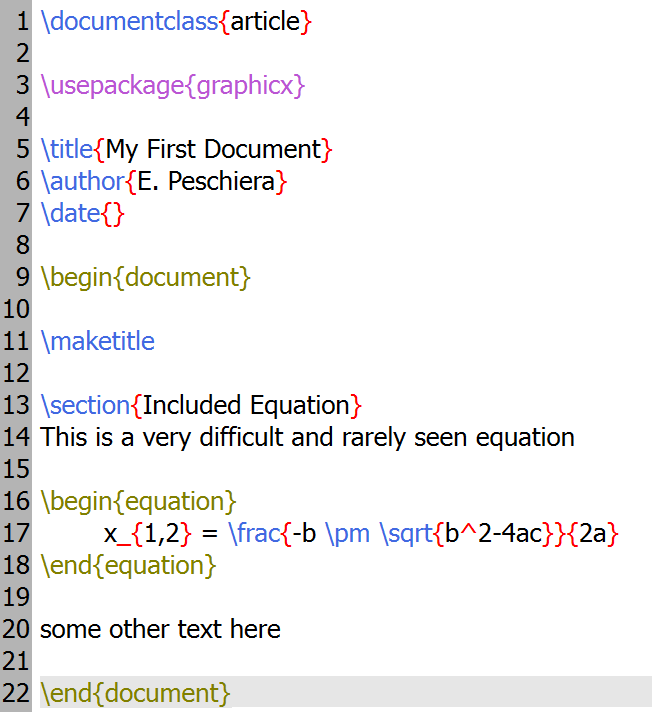
\includegraphics[scale=.4]{Figures/code4}
			\end{figure}
		\end{column}
		\begin{column}{.5\textwidth}
			\begin{figure}
			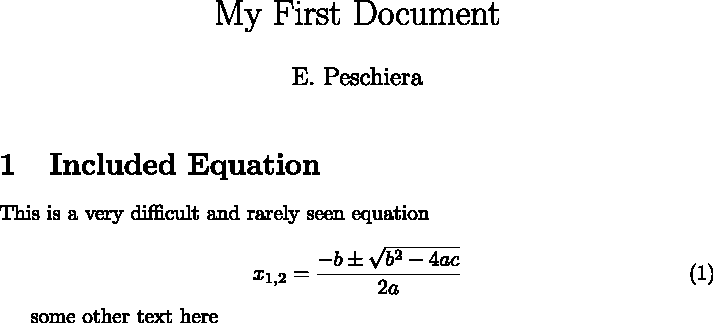
\includegraphics[width=.9\linewidth, frame, trim={-1cm -1cm -1cm -1cm},clip]{Figures/doc5}
			\end{figure}
		\end{column}
	\end{columns}	
\end{frame}

\begin{frame}[fragile]{Inserting an Equation}
In-line equation
\vspace{.5cm}
	\\An equation can also be in-line = inside the text
	\vskip.05\textheight
	This is enabled by using the math environment \texttt{\textcolor{red}{\$}...\textcolor{red}{\$}}
	\\\quad e.g., \texttt{Variable \$D\$ is calculated as \$D = S \textbackslash oplus d\_i\$ using the XOR operation.}
	\somespace
    \begin{center}
        Variable $D$ is calculated as $D = S \oplus d_i$ using the XOR operation.
    \end{center}
    
    \somespace
	Of course, not possible to refer to these equations as they do not have a number
\end{frame}